%   Filename    : chapter_4.tex 
\chapter{Research Methodology}
This chapter discusses the activities and methodologies employed by the researchers in conducting the study. These include the design of the study, persons involved, technical and software specifications, testing and operation, system implementation, methods and procedures.

\section{Design of the Study}

Aklan Animal Rehabilitation and Rescue Center is the province of Aklan’s only
animal shelter. This research focuses not only on the development of an animal
system, but also on the incorporation of gamification and log-in features to it.

Merriam-Webster defines gamification as the process of incorporating games
or game-like elements into something (such as a task) in order to increase participation. Zichermann and Cunningham (2011) believe that this framework
for understanding gamification is both powerful and adaptable, as it can be easily
applied to any problem that can be solved by influencing human motivation and
behavior.

The agile methodology is used by the researchers in the development of the
system. Agile Methodology is a practice that promotes continuous testing and
development throughout the development lifecycle of the system. In the Agile
model of software testing, both development and testing activities are carried out
concurrently. It is beneficial because the chosen animal rescue center will be given
frequent and early opportunities to inspect the product and make judgments and
revisions to the system before it will be implemented \cite{hamilton2021agile}.

\section{Persons Involved}

ADVISER. Being the co-author of the study, this person helps and supports
the researchers on the duration of the conduct of the study.

RESOURCE PERSON. Representative from Aklan Animal Rehabilitation and
Rescue Center is the resource person to ensure that the system is appropriate for
the users and the information is validated from the organization.

PROGRAMMER. The programmer develops the appropriate system to perform
methods and generate results in applying the gamification and log-in features.

RESEARCHERS. The researchers perform the handy activities from inquiry,
consultation, data gathering, system development, testing until the study is accomplished.

\section{System Specifications}

\subsection{Use Case Diagram}

\begin{figure}[h]
	\centering
	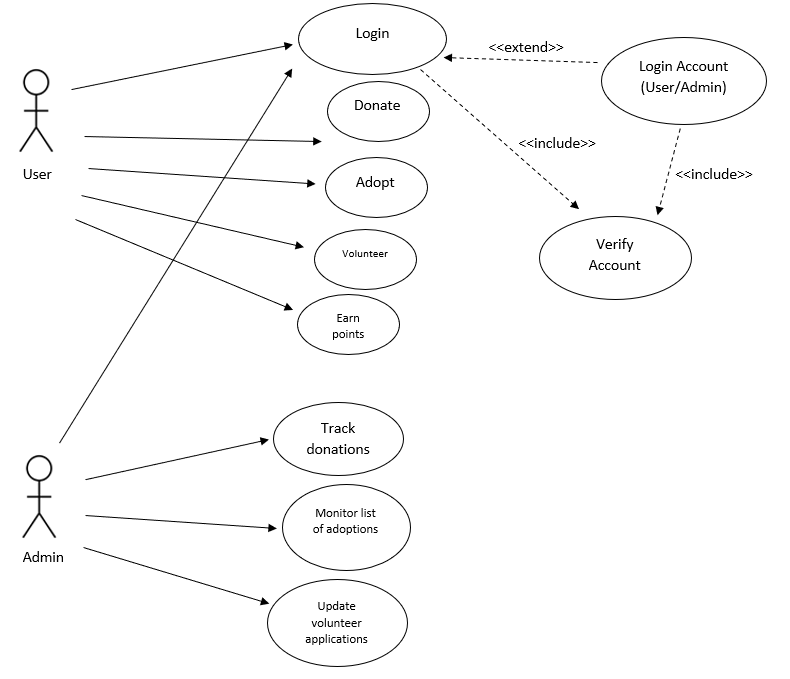
\includegraphics[width=10cm]{UseCase.png}
	\caption{The figure shows the use case diagram for the user and admin of the system.}
	\label{fig:usecase}
\end{figure}

\subsection{Functional Requirements}

The following system's functional requirements are applicable to both the random user and the system administrator:

\begin{enumerate}
	\item The system enables the user to create an account.
	
	\begin{itemize}
		\item The user will enter credentials such as username, email, and password.
		\item Verification of account by checking if:
			\begin{itemize}
			\item [--] Username is still available.
			\item [--] Email is active and not the same user.
			\item [--] Password includes needed characters.
			\item [--] Password is the same as the confirmed password.
			\end{itemize}
		\item Account is added to the database if the input credentials are valid. 
	\end{itemize}
	
	\item The system enables the user to log in to their accounts. 
	
	\begin{itemize}
		\item The user provides the username and password registered in the database.
		\item If credentials match an account registered in the database, access is granted; otherwise, access is denied.
	\end{itemize}

	\item The system enables the user to visit profile page.
	
		\begin{itemize}
			\item The profile page consists of three subpages:
			\begin{itemize}
				\item [--] main page
				\item [--] information page
				\item [--] contacts page
			\end{itemize}
			\item Information saved is displayed on the profile page.
		
		\end{itemize}
	\item The system enables user to modify profile information.
		
		\begin{itemize}
			\item Profile page is updated once new information is provided. 
			\item Old information is replaced in the database. 
		\end{itemize}
	\item The system enables user to log-out.
	
		\begin{itemize}
			\item The user will be logged out of the system when logout is clicked.
		\end{itemize}
\end{enumerate}

The following system's functional requirements are applicable to the random user:

\begin{enumerate}
	\item The system enables the user to own a virtual pet.
	\begin{itemize}
		\item The virtual pet is automatically owned by the user who has an account.
		\item The user can choose to have either a cat, a dog, or a rabbit as a virtual pet. 
		\item The virtual pet levels up its appearance once the user reached a certain number of virtual points. 
	\end{itemize}
	
	\item The system enables the user to earn virtual points.
	\begin{itemize}
		\item The virtual points serve as the basis for leveling up.
		\item Leveling up includes additional accessories for the virtual pet.
	\end{itemize}

	\item The system enables the user to adopt a pet.
	\begin{itemize}
		\item The list of animals available for adoption is available to the user.
		\item Names and descriptions of the animal are displayed for the users to choose who to adopt.
		\item An application form is needed to be filled out. 
		\item The information will be saved to the database. 
		\item The list of animals available for adoption is updated from the database.
		\item Virtual points is then earned by the user.
	\end{itemize}
	
	
	\item The system enables the user to volunteer at the Aklan Animal Rehabilitation and Rescue Center.
	\begin{itemize}
		\item An application form is needed to be filled out.
		\item The information will be saved to the database. 
		\item Virtual points is then earned by the user.
	\end{itemize}

	\item The system enables the user to donate to the Aklan Animal Rehabilitation and Rescue Center.
	
	\begin{itemize}
		\item The system will redirect the user to the AARRC main page.
		\item Mode of donation is provided to the user for donations.
		\item The user may choose what mode of donation to use. 
		\item Once donation is done, the information will be saved to the database. 
		\item The user will be redirected again to the system.
		\item Virtual points is then earned by the user.
	\end{itemize}
	
\end{enumerate}

The following system's functional requirements are applicable to the system administrator:

\begin{enumerate}
	\item The system enables the admin to monitor the list of animals available for adoption.
	\item The system enables the admin to monitor and update the list of volunteers for the rescue center.
	\item The system enables the admin to track donations made by the users. 
\end{enumerate}

\section{User Specifications}

The possible users of the study are the following:

RANDOM USER. This user can create an account to use the animal rescue system. This user can donate, adopt and volunteer to AARRC through this Rescue Pets animal rescue system. 

SYSTEM ADMINISTRATOR. The admin is responsible for managing the overall activity of the random users of the system. This user can track donations from the users, can monitor list of adopted animals from AARRC and can update volunteer applications for AARRC. 

THESIS ADVISER. The thesis adviser is the person with authority having the full knowledge on the special problem being conducted. The thesis adviser guides and provides meaningful advises to the researchers on the duration of the research activities.

RESEARCHERS. The researchers serve as the first user and beneficiary of the study. If implemented, the researchers are the primary user to engage in doing activities in the system such as donating, adapting and volunteering in AARRC.


\section{Technical and Software Specifications}

Various software applications used for the study are considered during
the planning and development phase conducted by the researchers.

\begin{itemize}
	\item Microsoft Windows 10 - this tool was used as the main
	operating system for developing the system.
	\item TexStudio and Microsoft Word - this tools were used for
	documentation purposes. They were used for the compilation of initial drafts and final copy of
	the SP document.
	\item Zoom application - was used for consultations and meeting with the adviser since
	face-to-face is not possible, this application was used by the researchers for
	consultations and meetings with the adviser.
	\item Github - Github was used for version control of the system and for easier
	collaboration. Github lets the researchers work together remotely.
	\item Adobe XD - Adobe XD is a prototyping tool for user experience and
	interaction designers. The tool was used for the initial prototype of the
	system.
	\item Sublime Text - it is a text editor used by the researchers in documenting the codes used to build the system
\end{itemize}

\section{Procedures}

\subsection{Development of the System}

This is the phase where the plan and design of the system are developed into a working system. 

Account creation is a method implemented in the study, so users must create an account before engaging with the system. The user can be a random user or a system administrator. In creating an account, the username, email, and password are asked from the users. 

Account verification is needed for the users to finally log in to the system. The database will be accessed if the following user is already available or not.

A virtual pet is automatically owned by the user once the account is created. The user can choose between a cat, a dog, or a rabbit as their virtual pet.

Gamification is applied in the system by recording the engagement of the user with the system by the use of virtual points. Every transaction made by the user has an equivalent number of virtual points. 

The user can donate, adopt, and volunteer to Aklan Animal Rehabilitation and Rescue Center through the system. The main database and the database of the virtual points are updated after every transaction of the user. 

The admin can track donations, monitor a list of volunteers, and animals available to adopt. The admin can access the activities of the user during the engagement with the system. 


\subsection{Testing and operation}

This is the phase that ensures the system’s operability and functionality.
Testing is necessary to elicit supplementary details and information to enhance
and improve the system.

People involved in the testing were asked to provide suggestions and recommendations
for enhancing and improving the system.

The study is tested by the following users: a) AARRC representative b) researcher’s
adviser c) researchers d) random users and e) system administrator.

\subsection{System Implementation}

The system’s possible implementation, as envisioned by the researchers, is
web-based. The mobile development of the system is further pursued based on
the researchers’ decision or can be done by future researchers who will conduct the
same study. Because the study’s focus is on the application of gamification and
log-in features to the animal rescue system, the study will be implemented after
careful and successful testing and operation of the system by domain experts.


